% !TEX program = pdflatex
% 光电探测器特性测量实验-实验报告
\documentclass[UTF8,10pt,a4paper]{article}
\usepackage{ctex}
% \catcode`\。=\active
% \newcommand{。}{.}
\newcommand{\CourseName}{近代物理实验}
\newcommand{\CourseCode}{PHYS1701}
\newcommand{\Semester}{2019-2020学年第学期}
\newcommand{\ProjectName}{实验报告}
\newcommand{\TimeType}{实验日期}
\newcommand{\Time}{2020. 5. 27(周三)}
\newcommand{\StudentName}{陈稼霖}
\newcommand{\StudentID}{45875852}
\usepackage[vmargin=1in,hmargin=.5in]{geometry}
\usepackage{fancyhdr}
\usepackage{lastpage}
\usepackage{calc}
\pagestyle{fancy}
\fancyhf{}
\fancyhead[L]{\CourseName}
\fancyhead[C]{\ProjectName}
\fancyhead[R]{\StudentName}
\fancyfoot[R]{\thepage\ / \pageref{LastPage}}
\setlength\headheight{12pt}
\fancypagestyle{FirstPageStyle}{
    \fancyhf{}
    \fancyhead[L]{\CourseName\\
        \CourseCode\\
        \Semester}
    \fancyhead[C]{{\huge\bfseries\ProjectName}\\
        \TimeType\ : \Time}
    \fancyhead[R]{姓名 : \makebox[\widthof{\StudentID}][s]{\StudentName}\\
        学号 : \StudentID\\
        成绩 : \underline{\makebox[\widthof{\StudentID}]{}}}
    \fancyfoot[R]{\thepage\ / \pageref{LastPage}}
    \setlength\headheight{36pt}
}
\usepackage{amsmath,amssymb,amsthm,bm}
\allowdisplaybreaks[4]
% \usepackage{multirow}
\usepackage{graphicx}
\usepackage{subfigure}
\begin{document}
\thispagestyle{FirstPageStyle}
\section{光电探测器光谱响应度的测量}
\subsection{实验步骤}
实际实验步骤与原讲义有差异,如下:
\begin{enumerate}
    \item \textbf{用汞灯定标}:通过光栅单色仪观察汞灯,调节光栅单色仪的旋钮直至观察到汞灯的波长为$436$ nm(紫色)和$546$ nm(绿色)的谱线,测得两条谱线对应的旋钮刻度分别为$4.270$ mm和$5.380$ mm,我们近似认为光栅单色仪选择的波长与光栅单色仪的旋钮刻度$x$之间成线性关系,即
    \begin{align}
        \lambda=436+\frac{546-436}{5.380-4.270}x,
    \end{align}
    其中波长$\lambda$以nm为单位,光栅单色仪的旋钮刻度$x$以mm为单位.
    \item \textbf{连接仪器}:将白光光源、调制盘、光栅单色仪、热释电探测器依次排列在一条直线上,将调制盘与光谱响应测试装置的“调制盘驱动”接口相连,将探测器与光谱响应测试装置的“输入”接口连接,将示波器与光谱响应测试装置的“选频输出”接口连接,打开白光光源、光谱响应测试装置和示波器的开关. 调整白光光源、调制盘、光栅单色仪、热释电探测器的相对位置,使示波器探测到正弦形式的信号且使信号的振幅最大.
    \item \textbf{测量光谱响应}:转动光栅单色仪的旋钮,记录光栅单色仪的旋钮刻度$x$,探测器的入射光波长$\lambda$和示波器上正弦信号的峰峰值,所得数据如表\ref{1-T}第三列.
    \item 用光电二极管代替热释电探测器,重复上一步操作,所得数据如表\ref{1-T}第五列.
\end{enumerate}

\section{数据处理}
\begin{enumerate}
    \item 用
    \begin{align}
        P(\lambda)=\frac{V_f(\lambda)}{R_fK_f},
    \end{align}
    计算入射单色光的功率,其中热释电探测器前放和主放放大倍数的成绩$K_f=100\times 300$,热释电探测器的响应度$R_f=900$ V/W,计算结果如表\ref{1-T}第四列.
    \item 绘制热释电探测器测量得到钨丝灯的光谱辐射特性曲线,如图\ref{1-F-1}.
    \item 用
    \begin{align}
        R(\lambda)=\frac{V(\lambda)}{P(\lambda)}=\frac{V_b(\lambda)/K_b}{P(\lambda)},
    \end{align}
    计算硅光电二极管的光谱响应度,其中硅光电二级管测量时总的放大倍数为$K_b=150\times 300$,计算结果如表\ref{1-T}第六列.
    \item 绘制硅光电二极管的光谱响应曲线,如图\ref{1-F-2}.
    \item 由图,白光光源的光谱在可见光区域内均有辐射功率分布,在波长$680$ nm附近为峰值;由图,硅光电二极管的光谱响应曲线在波长$420$ nm附近达到一个峰值,故其峰值响应波长为$\lambda_p\approx 420$ nm.
\end{enumerate}

\begin{table}[h]
    \centering
    \caption{光电探测器光谱响应度的测量实验数据记录表}
    \label{1-T}
    \begin{tabular}{|c|c|c|c|c|}
    \hline
    \begin{tabular}[c]{@{}c@{}}入射光波长\\ $\lambda$ / nm\end{tabular} & \begin{tabular}[c]{@{}c@{}}热释电探测器电压输出\\ $V_f$ / V\end{tabular} & \begin{tabular}[c]{@{}c@{}}入射光功率\\ $P(\lambda)$ / $\mu$W\end{tabular} & \begin{tabular}[c]{@{}c@{}}硅光电二极管探测器电压输出\\ $V_b$ / V\end{tabular} & \begin{tabular}[c]{@{}c@{}}硅光电二极管的光谱响应度\\ $R(\lambda)$ / (V/W)\end{tabular} \\ \hline
    300 & 2.16 & 0.0800 & 1.20 & 333 \\ \hline
    310 & 2.28 & 0.0844 & - & - \\ \hline
    320 & 2.30 & 0.0852 & 1.2 & 313 \\ \hline
    340 & 2.40 & 0.0889 & 1.28 & 320 \\ \hline
    360 & 2.52 & 0.0933 & 1.58 & 376 \\ \hline
    380 & 2.68 & 0.0993 & 2.40 & 537 \\ \hline
    400 & 3.72 & 0.138 & 3.84 & 619 \\ \hline
    420 & 5.00 & 0.185 & 5.20 & 624 \\ \hline
    440 & 7.20 & 0.267 & 7.20 & 600 \\ \hline
    460 & 11.9 & 0.441 & 8.50 & 429 \\ \hline
    480 & 18.4 & 0.681 & 10.3 & 336 \\ \hline
    500 & 25.1 & 0.930 & 12.6 & 301 \\ \hline
    520 & 33.4 & 1.24 & 17.5 & 314 \\ \hline
    540 & 43.2 & 1.60 & 21.4 & 297 \\ \hline
    560 & 53.4 & 1.98 & 25.4 & 285 \\ \hline
    580 & 63.6 & 2.36 & 28.8 & 272 \\ \hline
    600 & 77.6 & 2.87 & 30.4 & 235 \\ \hline
    620 & 92.0 & 3.41 & 32.8 & 214 \\ \hline
    640 & 104 & 3.85 & 33.2 & 192 \\ \hline
    660 & 114 & 4.22 & 32.6 & 172 \\ \hline
    680 & 118 & 4.37 & 32.0 & 163 \\ \hline
    700 & 112 & 4.15 & 29.8 & 160 \\ \hline
    \end{tabular}
\end{table}

\begin{figure}[h]
	\centering
	\subfigure[热释电探测器测量得到的钨丝灯的光谱辐射特性曲线.]{
	\label{1-F-1}
	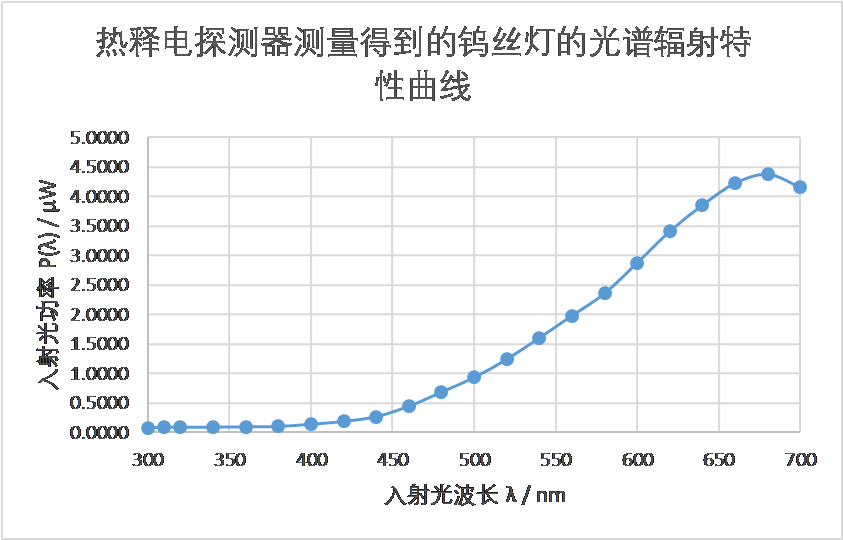
\includegraphics[width=.45\textwidth]{1-F-1.png}}
	\subfigure[硅光电二极管的光谱响应曲线.]{
	\label{1-F-2}
    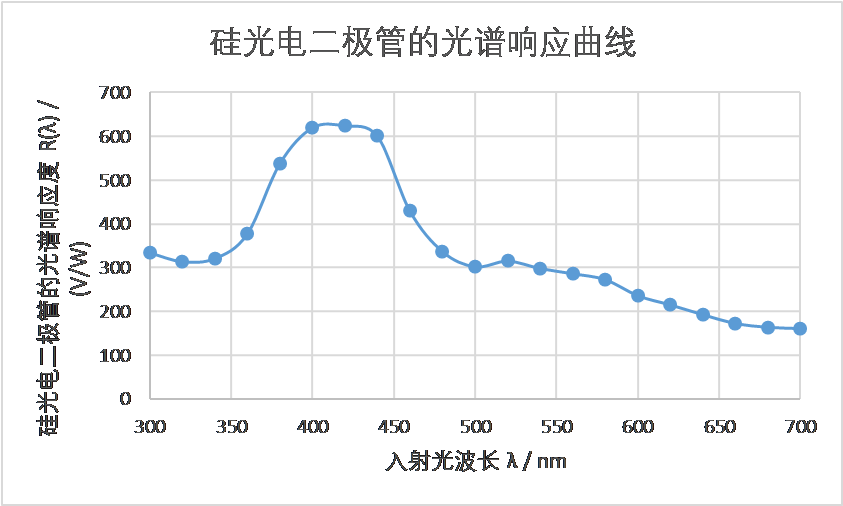
\includegraphics[width=0.45\textwidth]{1-F-2.png}}
    \caption{}
\end{figure}

\subsection{思考题}
\begin{enumerate}
    \item 单色仪入射狭缝和出射狭缝的宽度分别控制着哪些物理量?测量时开大些好还是开小些好?\\
    单色仪入射狭缝和出射狭缝的宽度都影响着单色仪对透射光波长的分辨率和透射光的强度:根据单缝衍射公式,中央明条纹的角宽度$\Delta\theta$为
    \begin{align}
        a\sin\Delta\theta=\lambda\quad\Longrightarrow\quad\Delta\theta=\frac{\lambda}{a},
    \end{align}
    其中$a$为缝宽,$\lambda$为入射光的波长,入射缝宽越小,衍射越明显,也就是说不同波长的光束的角度差异越大,而出射缝宽越小,也就是光束允许的传播角度范围越小,因此透过的光的单色性越好. 因此入射和出射缝宽越小,单色仪分辨率越高. 但是入射和出射缝宽越小,能够透过单色仪光的越少,探测到的信号越小,这样一来可能导致信噪比降低.\\
    测量时,应当在保证探测到的信号信噪比足够的前提下,尽可能缩小单色仪入射和出射狭缝的宽度.
    \item 如果在测量过程中,用热释电器件和光电二极管测量时,二者光源强度不一致是否能保证结果的正确性?如果二者的调制频率不同呢?\\
    这个问题需要分类讨论:如果光源强度过强,导致超出探测装置的量程,或光源强度过弱,导致探测装置无法探测到信号,或光源的谱线形状并不是随着光源的温度呈等比例变化的,就无法保证结果的正确性;如果光源谱线形状是随着光源的强度呈现等比例变化(光谱形状不变,仅绝对强度发生变化),且探测器仍然可以在量程内准确测得信号,则测得的硅光二极管光谱响应度是不准确的,但是得到的峰值响应波长仍然是准确的.\\
    这里有必要先解释一下调制器的作用:(它的作用有点类似锁相放大)调制器是一个带有通光孔的圆盘,测量时驱动圆盘转动,从而使通过的光强度呈现周期性的变化,转换成示波器的电信号就是随时间呈现正弦(也可能不是标准的正弦)形式变化的曲线,其中电信号的极小值对应的是光源发出的光束完全被调制器所遮挡时探测器测量到的信号(也就是一些环境光带来的噪声),电信号的极大值对应的是光源发出的光束不被圆盘遮挡时探测器测量到的信号(既包括光源发出的光束产生的电信号,也包括环境光带来的噪声),电信号极大值和极小值之差(也就是我们在实验中测量的峰峰值)就是光源发出的光被探测器接收,通过这样一种取差的方式,我们就可以将环境光带来的噪声去除. 因此即使调制频率不同,得到的电信号的峰峰值不会受到影响,结果仍然是正确的.
\end{enumerate}

\newpage
\section{光电探测器响应时间的测试}
\subsection{实验数据}
\begin{enumerate}
    \item \textbf{用脉冲法测量光电二极管的响应时间}
    \begin{table}[h]
        \centering
        \caption{硅光电二极管的响应时间与偏置电压的关系}
        \label{2-T-1}
        \begin{tabular}{|c|c|c|c|c|}
        \hline
        偏置电压 $E$ / V & 0 & 5 & 10 & 15 \\ \hline
        响应时间 $t_r$ / s & 无响应(可认为响应时间无穷大) & 5.300E-05 & 6.400E-05 & 4.500E-05 \\ \hline
        \end{tabular}
    \end{table}
    \\(预期偏置电压为$10$V时,响应时间应该在$5.300\times 10^{-5}\sim 4.500\times 10^{-5}$s之间,这里可能发生了读数错误)
    \begin{table}[h]
        \centering
        \caption{硅光电二极管的响应时间与负载电阻的关系}
        \label{tab:my-table}
        \begin{tabular}{|c|c|c|c|c|c|}
        \hline
        负载电阻 $R_L$ / $\Omega$ & 500 & 100 & 10000 & 50000 & 100000 \\ \hline
        响应时间 $t_r$ / s & 3.400E-05 & 3.200E-05 & 4.500E-05 & 1.100E-04 & 1.960E-02 \\ \hline
        \end{tabular}
    \end{table}
    \begin{figure}[h]
        \centering
        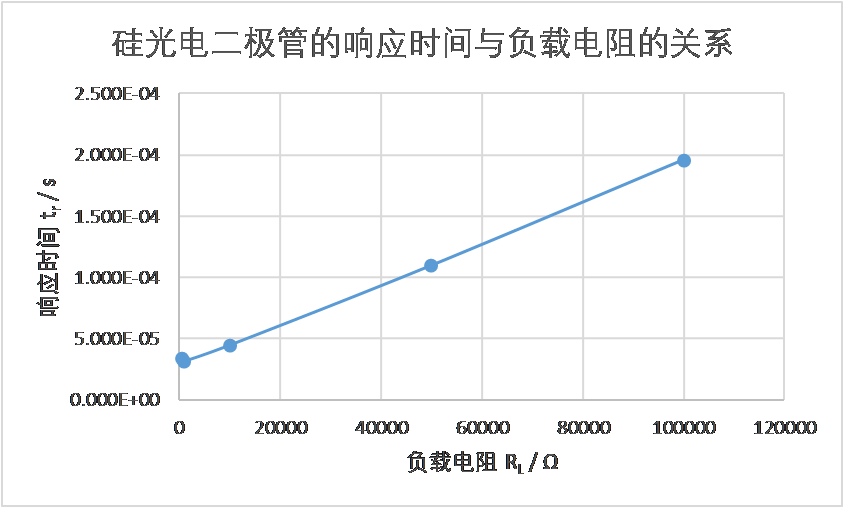
\includegraphics[width=.45\textwidth]{2-F-2.png}
        \caption{硅光电二极管的响应时间与负载电阻的关系}
        \label{2-F-2}
    \end{figure}
    \item \textbf{用幅频特性法测量CaSe光敏电阻的响应时间}:
    \begin{table}[h]
        \centering
        \caption{CdSed光敏电阻的输出电压与光波信号频率之间的关系}
        \label{2-T-3}
        \begin{tabular}{|c|c|c|c|c|c|c|}
        \hline
        光波信号频率 f / Hz & 9.756 & 24.87 & 35.84 & 95.23 & 148.1 & 225.5 \\ \hline
        示波器峰峰值 / V & 13.2 & 9.80 & 8.40 & 4.50 & 3.40 & 2.30 \\ \hline
        输出电压 V / V & 6.60 & 4.90 & 4.20 & 2.25 & 1.70 & 1.15 \\ \hline
        \end{tabular}
        \end{table}
        \\我们本可以用式(2-3)
        \begin{align}
            \tau=\frac{1}{2\pi}\sqrt{\frac{V_1^2-V_2^2}{(V_2f_2)^2-(V_1f_1)^2}}
        \end{align}
        来计算响应时间,但这样就浪费了测量的多组数据,因此不是最好的方法. 更好的方法是利用式(2-2)
        \begin{align}
            V(\omega)=\frac{V_0}{(1+\omega^2\tau^2)^{1/2}},
        \end{align}
        变形一下可以得到
        \begin{align}
            \frac{1}{V^2(\omega)}=\frac{1+\omega^2\tau^2}{V_0^2},
        \end{align}
        我们可以做$\frac{1}{V^2(\omega)}$关于$\omega^2$的散点图并线性拟合,如图\ref{2-F-3},拟合得到的直线斜率为$\frac{\tau^2}{V_0^2}=3.59\times 10^{-7}\text{s}^2/\text{V}^2$,截距为$\frac{1}{V_0^2}=0.0386\text{V}^{-2}$,两者相除开方得到$\tau=0.00305$s.
        \begin{figure}[h]
            \centering
            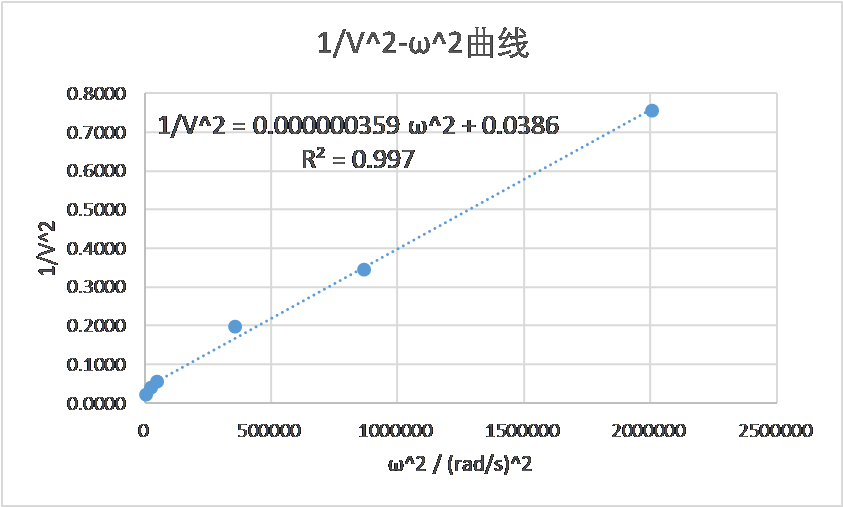
\includegraphics[width=.45\textwidth]{2-F-3.png}
            \caption{$\frac{1}{V^2}$--$\omega^2$曲线.}
            \label{2-F-3}
        \end{figure}
        \item \textbf{用截止频率测量CdSe光敏电阻的响应时间}:正弦信号频率的最低频率为$9.756$ Hz,其对应的信号峰峰值为$13.2$ V,增加正弦信号的频率至光敏电阻探测到的信号峰峰值为$9.33$ V,此时对应的调制频率$f_c=27.47$ Hz,故CaSe的响应时间为
        \begin{align}
            \tau=\frac{1}{2\pi f_c}=0.005794s
        \end{align}
\end{enumerate}

\subsection{数据分析}
\begin{enumerate}
    \item \textbf{光电二极管的响应时间与负载电阻和偏置电压的关系}:偏置电压越大,光电二极管的响应时间越短. 原因如下:用脉冲法测量光电二级管的响应时间的实验电路图如\ref{2-F-4},直流反向偏压电源、负载电阻和光电二极管三者串联,其中偏压电源的正极连接二极管的N端,负极连接二极管的P端. 反向偏压在二极管中产生了由P端指向N端的电场,从而增强了耗尽区原有的电场. 此时电脉冲驱动光电探测器时间常数测试实验箱中的光电器件发光管(这是另一个电路了,没有画在图中)瞬间产生光,光照射二极管,使得二极管耗尽区附近的原子被激发,产生电子空穴对,在当地电场的作用下,电子向N端移动,而空穴向P端移动,从而相互分离成为载流子. 反向偏压越强,耗尽区电场越强,激发得到的电子空穴对可以越快地被拉开,从而更快地产生载流子,产生响应电流,也就是响应时间越短.\\
    负载电阻越大,光电二极管的响应时间越长. 这是因为负载电阻和二极管串联分压,负载越大,分到电压越大,二极管分到电压越小,从而上面所提到的将激发得到的电子空穴对拉开成为载流的速率越慢,响应时间越长.
    \begin{figure}[h]
        \centering
        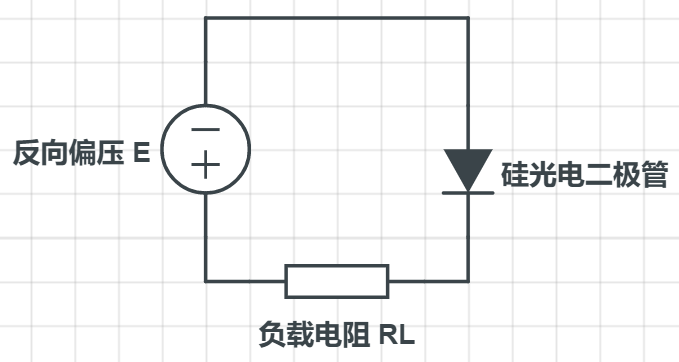
\includegraphics[width=.45\textwidth]{2-F-4.png}
        \caption{测量光电二极管响应时间电路图.}
        \label{2-F-4}
    \end{figure}
    \item 实验步骤中并没有用脉冲响应法测量CaSe光敏电阻的响应时间的内容,这是因为在实验原理中已经提到过,由于光电探测器惰性的存在,其响应度不仅与入射辐射的波长有关,而且还是入射辐射调制频率(入射光强信号的波形)的函数,用脉冲响应法测量响应时间时使用的波形是脉冲波,用幅频特性法测量响应时间时使用的波形是正弦波,这两种不同的波形必然导致CaSe不同的响应表现,对应的响应时间实际上根本没有比较的意义.
    \item 用截止频率法得到的响应时间相对幅频特性法所得值差了将近一倍,但尚处于同一个数量级,我们认为幅频法用了6个光波信号频率下采集的数据点,应该更为准确.
    \item \textbf{三种方式的特点}:脉冲响应法和另外两种方法测量的分别是脉冲形式和正弦形式的入射辐射激励下光电元件的响应时间,脉冲响应法和截止频率法的操作较为简单,但是它们只能得到一个数据值,因而误差可能较大,而幅频特性法如上面所进行的数据处理那样,可以测量在不同频率下的多个数据点,然后拟合出响应时间,因而虽然操作更为复杂,但可能具有更高的精度.
\end{enumerate}
\end{document}